
\section{EASIROCの内部動作}
ボードの内部には2つのEASIROCチップが埋まっており、最大で 64チャンネルの MPPC を同時に読み出すことができる。
EASIROC チップからのアナログ信号は4つの ADC でデジタル信号に変換、Discriminator 出力は MHTDC 及び Scaler に入力され、Gatherer、Sender、SiTCP を介してデータ取得PC(DAC)に渡される。
DAC と EASIROC ボード は Ethernet ケーブルでつながっている。必要な動作電圧は +6 V であり、NIMビンから供給可能である。
\begin{figure}[H]
\begin{center}
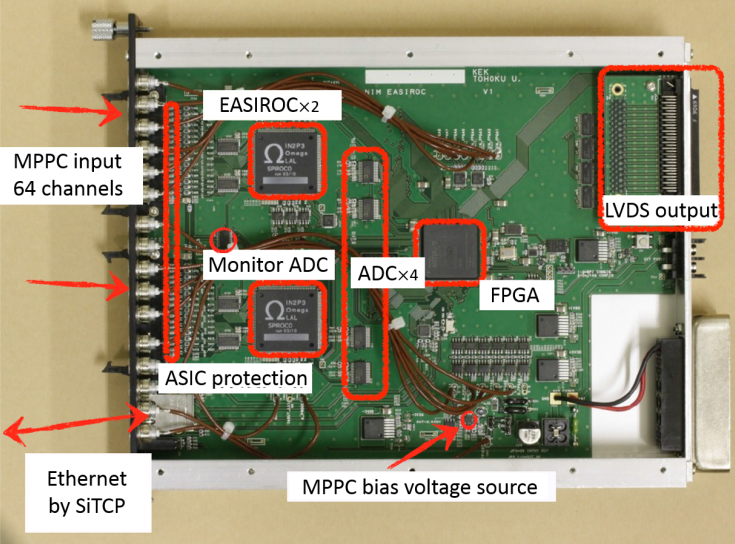
\includegraphics[width = 10.0cm, bb= 0 0 735 544]{2.png}
\end{center}
\caption{NIM-EASIROCボードの側面}
\label{fig:}
\end{figure}

\begin{figure}[H]
\begin{center}
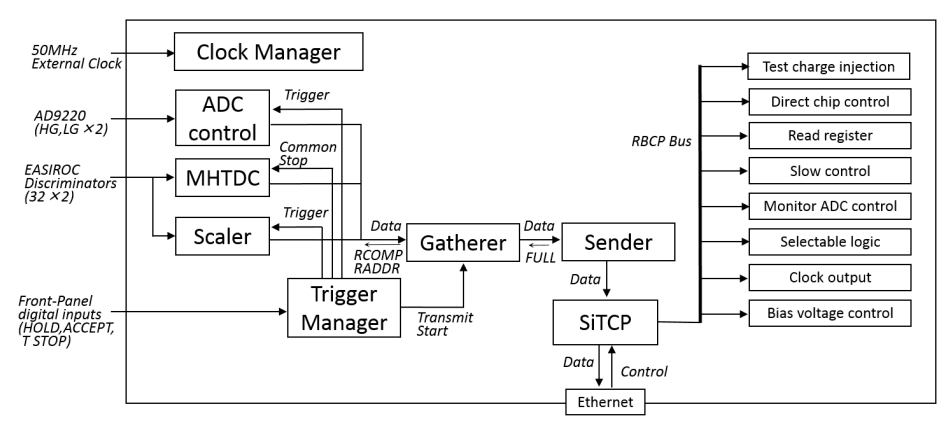
\includegraphics[width = 10.0cm, bb= 0 0 952 424]{3.png}
\end{center}
\caption{NIM-EASIROCボードの回路イメージ}
\label{fig:}
\end{figure}

\begin{figure}[H]
\begin{center}
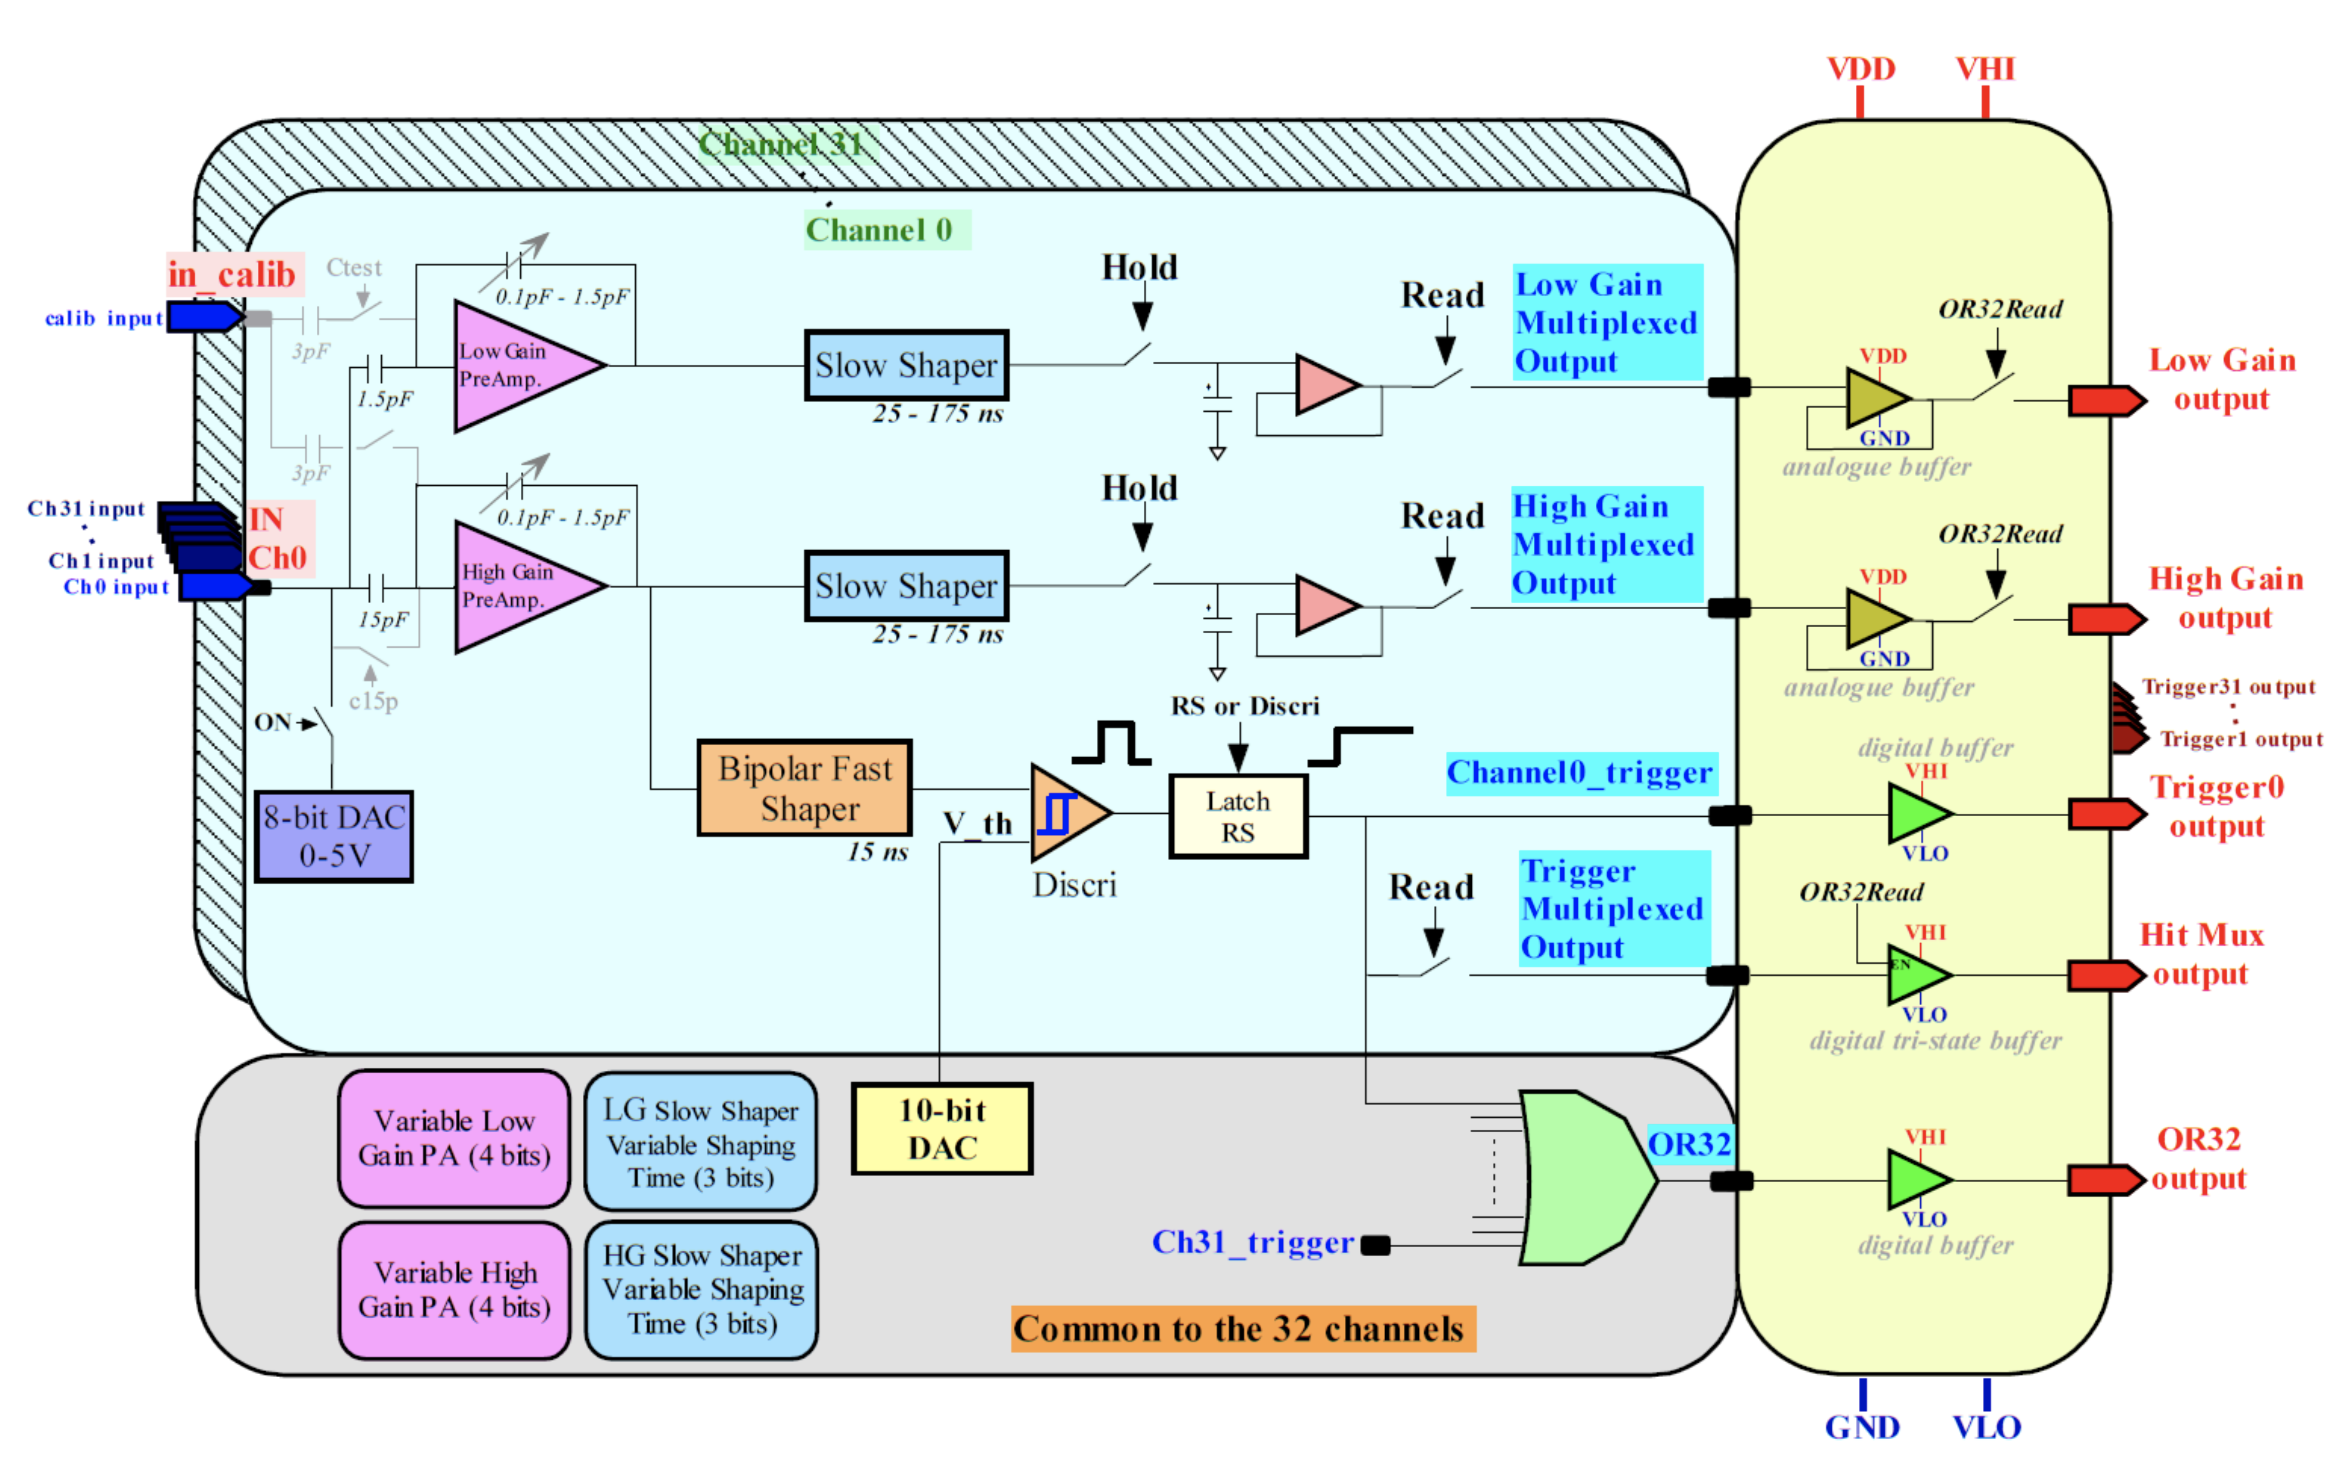
\includegraphics[width = 13.0cm, bb= 0 0 1167 735]{5.png}
\end{center}
\caption{EASIROC チップのブロックダイアグラム}
\label{fig:}
\end{figure}

アナログ信号の変換手順は以下のようになる。
\begin{enumerate}
\item Low 及び High 二つの異なるゲインを持つプリアンプにより電荷が積分・増幅される
\item プリアンプ出力は Fast shaper 及び Slow shaper に入力される
\item Fast shaper に入った信号は時定数 15 ns で整形され、Discriminator の Threshold を超えた場合にデジタル信号に変換される
\item Slow shaper に入った信号は時定数 25 - 175 ns で整形され、HOLD 信号を受け取った瞬間の電圧値が保持・記録される
\end{enumerate}

